% !TeX root = /../pythonTutorial.tex
\chapter{Ein- und Ausgabe}
\label{inputOutput}

In diesem Kapitel gehen wir auf die Eingabe und Ausgabe von Informationen ein. Wie etwa der Nutzer mit dem Programm kommunizieren kann, aber auch das Einlesen und Bearbeiten von Dateien werden hier genauer betrachtet.

Die Ausgabe �ber die Konsole ist uns schon als \emph{print()}-Befehl begegnet. Diesen schauen wir uns nun etwas genauer an.


% !TeX root = ../../pythonTutorial.tex
\section{Konsolenausgabe mit print()}
\label{printInOut}

Die \emph{print()}-Funktion hat vielerlei Nutzen und wird entsprechend oft verwendet. Daher ist es definitiv sinnvoll, sich mit ihr vertraut zu machen.

\begin{lstlisting}[language=Python, label=printInOut:lst:printDefault]
# die Print-Methode

print(value1, value2, ..., sep=" ", 
    end="\n", file=sys.stdout, flush= false))
\end{lstlisting}

In Listing (\ref{printInOut:lst:printDefault}) sind die Parameter von \emph{print()} zu sehen. Die auszugebenden Werte stehen an erster Stelle (value1, value2, ...), hierbei handelt es sich um eine beliebige Anzahl an Werten. Der Parameter \emph{sep} bildet den Seperator zwischen den Werten und hat als Standardwert das Leerzeichen.
\randnotiz{Seperator}
In Listing \ref{printInOut:lst:printSeperator} k�nnen wir sehen, dass wir durch Angabe eines Seperators eine bessere Lesbarkeit erreichen k�nnen.

\begin{lstlisting}[language=Python, label=printInOut:lst:printSeperator]
# die Print-Methode mit Seperator

print(1,2,3)
# Ausgabe: 1 2 3

print(1,2,3, sep=" | ")
# Ausgabe: 1 | 2 | 3
\end{lstlisting}

Nach dem Seperator folgt der \emph{end}-Parameter, dieser f�gt standardgem�� einen Zeilenumbruch (\textbackslash n) an das Ende der Ausgabe.
\randnotiz{End-Angabe}

\begin{lstlisting}[language=Python, label=printInOut:lst:printEnd]
# die Print-Methode mit End-Angabe

print("Satz mit Zeilenumbruch")
print("N�chster Satz")
# Ausgabe:
# Satz mit Zeilenumbruch
# N�chster Satz

print("Satz mit Punkt und Leerzeichen." , end=". ")
print("N�chster Satz)
# Ausgabe: 
# Satz mit Punkt und Leerzeichen. N�chster Satz
\end{lstlisting}

Der \emph{file}-Parameter bestimmt den Datenstrom (\emph{Stream}) f�r den Output. In \emph{sys.stdout} steht f�r die Konsole. 
\randnotiz{Output-Stream}
M�chten wir den Output bspw. in eine Textdatei schreiben, dann k�nnen wir diese als Ziel des Datenstroms festlegen.

\begin{lstlisting}[language=Python, label=printInOut:lst:printFile]
# die Print-Methode mit Ausgabe in Textdatei

# open() -> festlegen einer Textdatei als Stream
# "w" steht f�r 'write' und gibt an,
# dass wir etwas in die Datei schreiben m�chten

txtFile = open(beispielText.txt, "w")
print("Hello, World.", file="txtFile")
txtFile.close()
# close() schlie�t den Stream
\end{lstlisting}





%% !TeX root = ../../pythonTutorial.tex
\section{Formatierung von Strings}
\label{formatInOut}

Es w�re sicherlich hilfreich, wenn wir die String-Ausgaben nach belieben formatieren k�nnten. Bisher haben wir den Seperator von \emph{print()} kennengelernt - dieser ist von seiner Funktionsweise jedoch stark beschr�nkt. Python bietet uns hierf�r die \emph{format()}-Methode an, vorher betrachten wir aber die Modulo-Arithmetik und machen uns mit den Formatierungszeichen vertraut.
 
Mittels Modulo-Arithmetik \randnotiz{Modulo-
Arithmetik} leiten wir ein Formatierungszeichen ein. Dieses gilt als Platzhalter f�r einen Wert.

\begin{lstlisting}[language=Python, label=formatInOut:lst:modulo]
# Modulo-Arithmetik

print("K�rper: %s , Fl�che: %f m" %
	('Dreieck', 42.6))
	
# Ausgabe:
# K�rper: Dreieck , Fl�che: 42.6
\end{lstlisting}

Bei "'K�rper"' setzen wir den ersten Platzhalter mit "'\%s"'. Die Reihenfolge der Platzhalter setzt fest, welcher Wert anschlie�end eingebunden wird. Der erste Platzhalter tr�gt also den ersten Wert, der nach dem Ausgabetext folgt, der zweite den zweiten und so weiter.

\warning{Die einzusetzenden Werte werden nach dem String mittels Modulo als Tupel festgelegt!}

Das Formatierungszeichen nach dem Modulo bestimmt den Datentyp des Wertes.
Bei "'s"' handelt es sich um einen String, bei "'f"' um ein \emph{float}.
In folgender Tabelle sind die m�glichen Formatierungszeichen aufgelistet.

\begin{figure}
	\caption{Formatierungszeichen und ihre Bedeutung \cite{pythonFormat}}
	\centering
	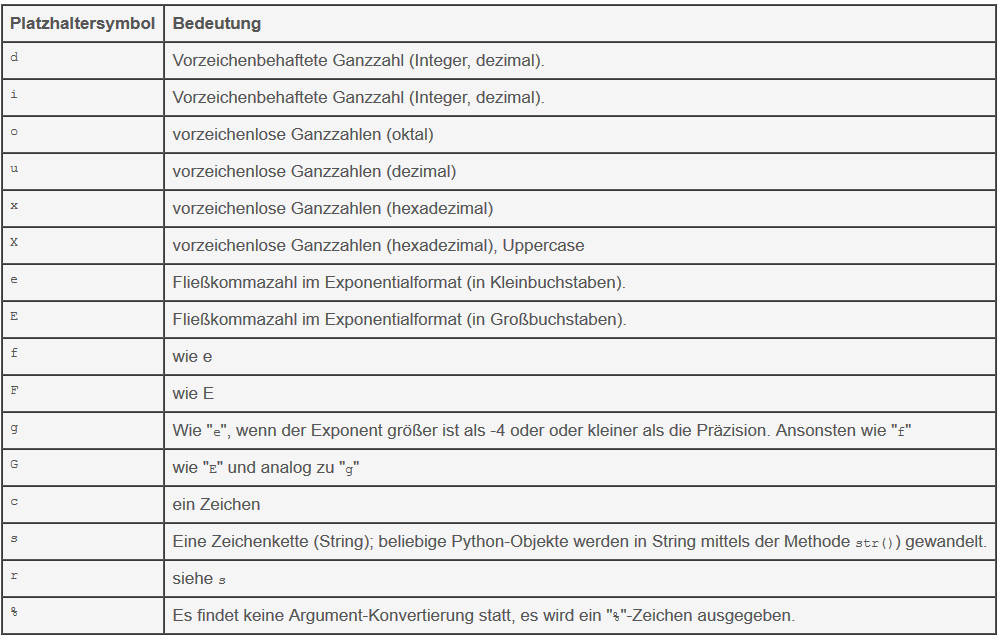
\includegraphics[width=\textwidth]{chapters/inputOutput/FormatierungSymbole.png}
\end{figure}

Was ist jedoch, falls die Ausgabe eine bestimmte L�nge haben soll?
Mit Hilfe der Syntax der Modulo-Arithmetik k�nnen wir dieses Problem l�sen.

 \begin{lstlisting}[language=Python, label=formatInOut:lst:syntax]
 # Modulo-Arithmetik Syntax
 
%[Flag][Minimum der Gesamtl�nge].[Pr�zision][Typ]
 \end{lstlisting}
 
 Das Minium der Gesamtl�nge bringt gro�e Vorteile mit sich, wenn wir z.B. einen linksb�ndigen Text ausgeben wollen. Alle Ausgaben, die k�rzer als das vorgegebene Minimum sind, werden mit Leerzeichen aufgef�llt.
 
 \warning{Es handelt sich hierbei um das Minimum der Gesamtl�nge. Alle Ausgaben die gr��er sind, werden nicht beschr�nkt und in voller L�nge ausgegeben!}
 
 Mittels Punkt k�nnen wir folgend die Pr�zision einstellen, was bei einem \emph{Float}-Datentyp die Nachkommastellen bestimmt. Alle Zahlen werden zu der angegebenen Nachkommastelle aufgerundet!
 
 \begin{lstlisting}[language=Python, label=formatInOut:lst:precision]
 # Modulo-Arithmetik Pr�zision
 
print("Eine Zahl %f" % (1.234))
print("Eine gerundete Zahl %.2f)

# Ausgabe:
# Eine Zahl 1.234
# Eine gerundete Zahl 1.23
\end{lstlisting}
 
\subsection{Formatierung mit format()}

Python bietet uns f�r die Formatierung von String-Elementen die Methode \emph{format()}.

 \begin{lstlisting}[language=Python, label=formatInOut:lst:formatMethod]
# Syntax der format()-Methode 

string.format(par0, par1, ..., key0=val0, key1=val1, ...)
\end{lstlisting}

\emph{format()} ersetzt markierte Stellen im gegebenen String durch angegebene Werte (Parameter in \emph{format()}) und liefert diesen zur�ck.
Die Stellen werden durch geschweifte Klammern markiert und mittels Modulo-Arithmetik pr�zisiert. In der geschweiften Klammer geben wir als erstes den Index (oder das Schl�sselwort) des Parameters an.

 \begin{lstlisting}[language=Python, label=formatInOut:lst:formatString]
# format() mit gegebenem String 

str = "Hallo, {0:s} und {1:s}"
print(str.format("Rainer", "Denis"))
# Ausgabe: 
# Hallo, Rainer und Denis

print(str)
# Ausgabe:
# Hallo, {0:s} und {1:s}

# format() ver�ndert den String nicht,
# sondern liefert den ver�nderten Wert zur�ck

str = str.format("Rainer", "Denis")
print(str)
# Ausgabe: 
# Hallo, Rainer und Denis

# der Wert von 'str' wurde durch den R�ckgabewert
# von format() �berschrieben!

str = "Hallo, {1:s} und {0:s}"
str.format("Rainer", "Denis")
print(str)
# Ausgabe:
# Hallo, Denis und Rainer

# in 'str' wurde der angegebene Index vertauscht

str = "Hallo, {r:s} und {d:s}"
print(str.format(r = "Rainer", d ="Denis"))
# Ausgabe: 
# Hallo, Rainer und Denis

# Angabe von Schl�sselwort-Parametern
\end{lstlisting}

\warning{M�chte man geschweifte Klammern ausgeben, dann werden diese doppelt geschrieben ("'\{\{"' und "'\}\}"')}

Die \emph{format()}-Methode bietet uns au�erdem Ausrichtungsoptionen, was zu besserer Lesbarkeit beitragen kann. Somit k�nnen wir bspw. Werte links- oder rechtsb�ndig ausgeben. Hierf�r gibt man die Formatierungsanweisung an und den Wert des Abstandes bzw. der Gr��e des Platzhalters. Ist das Wort zu kurz, wird der restliche Platz mit Leerzeichen aufgef�llt.

\begin{tabular}{|c | p{8cm}|}
	\hline
	Formatierungsanweisung & Bedeutung \\
	\hline
	< & Text wird linksb�ndig ausgelegt \\
	> & Text wird rechtsb�ndig ausgelegt \\
	\hline
\end{tabular}


\begin{lstlisting}[language=Python, label=formatInOut:lst:formatAlignment]
# Ausrichtung mit Formatierungsanweisung

# linksb�ndig
str = "{0:<10s} {1:d}"
print(str.format("Viereck", 4))
print(str.format("F�nfeck", 5))
print(str.format("Sechseck", 6))

# Ausgabe:
# Viereck    4
# F�nfeck    5
# Sechseck   6


# rechtsb�nding
str = "{0:>10s} {1:d}"
print(str.format("Viereck", 4))
print(str.format("F�nfeck", 5))
print(str.format("Sechseck", 6))

# Ausgabe:
#    Viereck 4
#    F�nfeck 5
#   Sechseck 6
\end{lstlisting}

Python bietet uns f�r \lstinline{Dictionaries} einen einfachen Weg, diese mittels \emph{format()} und der Nutzung von Schl�sselwort-Parametern, auszugeben. 
	
\begin{lstlisting}[language=Python, label=formatInOut:lst:formatDict]
# Formatierung eines Dictionarys

dictMath = {"Dreieck" : "3", 
	   "Viereck" : "4", 
	   "F�nfeck" : "5",

str = "{body}: {corners}"

for geoBody in dictMath
    print(str.format(body=geoBody, 
                     corners=dictMath[geoBody]))
    
# Ausgabe:
# Dreieck: 3
# Viereck: 4
# F�nfeck: 5
\end{lstlisting}



% !TeX root = ../../pythonTutorial.tex
\section{Konsoleneingabe mit input()}
\label{inputInOut}

Mit Hilfe von \lstinline$input()$ erlauben wir dem Nutzer Eingaben �ber die Konsole. Somit erhalten wir den ersten Grad an Interaktion zwischen Nutzer und Programm.

\begin{lstlisting}[language=Python, label=inputInOut:lst:inputDefault]
# die input-Methode

input(prompt)
\end{lstlisting}

Sobald \lstinline$input()$ aufgerufen wird, wartet das Programm mit dem weiteren Ablauf, bis der Nutzer seine Eingabe mit der Eingabetaste best�tigt.
Die \lstinline$input()$-Methode liefert den eingegebenen Wert als String zur�ck.
Damit der Nutzer wei�, was er denn eingeben muss, bietet \lstinline$input()$ den optionalen Standard-Parameter \lstinline$prompt$ an - hierbei handelt es sich um einen leeren String.
Geben wir \lstinline$prompt$ nun einen Wert, wird dieser dem Nutzer f�r die Eingabe angezeigt.

\begin{lstlisting}[language=Python, label=printInOut:lst:inputPrompt]
# die input-Methode mit prompt-Angabe

userName = input("Geben Sie Ihren Namen ein.")
print("Hallo, " + userName)
\end{lstlisting}

\warning{Der Eingabewert des Nutzer liefert immer einen String zur�ck.
Bei gew�nschtem Datentyp, muss \emph{gecasted} werden!}

\kontrollfrage{
	\item[\kontroll] Wie verh�lt sich das Programm bei Aufruf der \lstinline$input()$-Methode?
	\item[\kontroll] Welchen Wert liefert \lstinline$input()$ zur�ck? Um was f�r einen Datentyp handelt es sich?
	\item [\kontroll] Welchen Effekt hat die Angabe des \lstinline{prompt}-Parameters?
}

Bei primitiven Datentypen ist das Umwandeln recht einfach. Bei nicht-primitiven kann es jedoch zu �berraschungen kommen.

\begin{lstlisting}[language=Python, label=printInOut:lst:inputCast]
# die input-Methode mit Typ-Umwandlung

summe = int(input("2 + 3 = "))
print(summe, type(summe), sep=" - ")
# Eingabe: 5
# Ausgabe: 5 - <class 'int'>

geoKoerper = list(input("Geben Sie einige" +
			"geometrische K�rper an"))
print(geoKoerper)
# Eingabe: ["Dreieck", "Viereck"]
# Ausgabe: [' ', '[', '"', 'D', 'r', 'e', 
	'i', 'e', 'c', 'k', '"', ',', 
	' ', '"', 'V', 'i', 'e', 'r', 
	'e', 'c', 'k', '"', ']']
			
print(type(geoKoerper[0]))
# Ausgabe: <class 'str'>

\end{lstlisting}

Python wandelt den String in eine Liste um, jedoch nimmt es jedes einzelne Zeichen der Eingabe als Listenelement. Dies kann durchaus n�tzlich sein, verfehlt hierbei aber das Ziel. Um die geometrischen K�rper als Elemente zu erhalten, nutzen wir die \lstinline$eval()$-Funktion.
\randnotiz{\lstinline$eval()$}
Hierbei wird die Eingabe interpretiert und der entsprechende Datentyp zur�ckgeliefert (Evaluierung).

\tip{eval() funktioniert auch bei anderen Collections!}

\begin{lstlisting}[language=Python, label=printInOut:lst:inputEval]
# die input-Methode mit eval()

geoKoerper = eval(input("Geometrische K�rper: "))
print(geoKoerper)
# Eingabe: ["Dreieck", "Viereck"]
# Ausgabe: ['Dreieck', 'Viereck']
\end{lstlisting}


\kontrollfrage{
	\item[\kontroll] Wie verh�lt sich der R�ckgabewert von \lstinline$input()$, wenn man ihn zu einer Liste umwandelt?
	\item[\kontroll] Welche Methode bietet uns Python an, um den R�ckgabewert wie gew�nscht zu erhalten?
}
